\begin{figure}[H]
    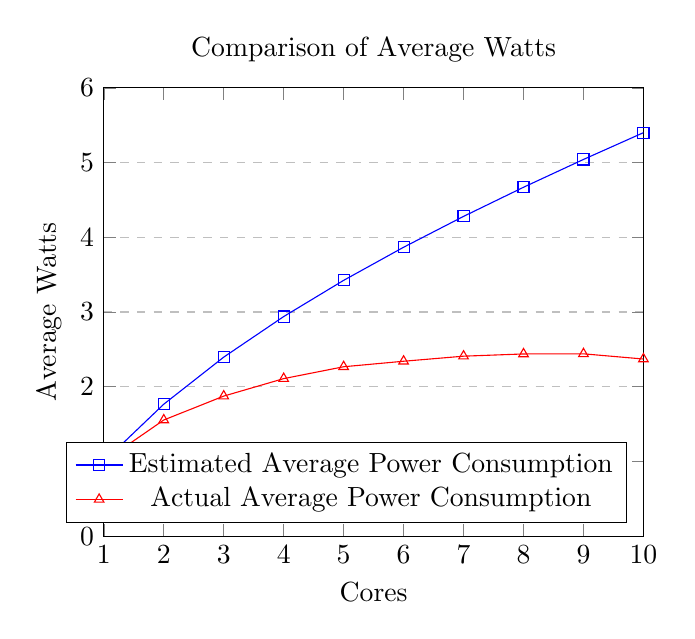
\begin{tikzpicture}
    \begin{axis}[
        title={Comparison of Average Watts},
        xlabel={Cores},
        ylabel={Average Watts},
        xmin=1, xmax=10,
        ymin=0, ymax=6,
        xtick={1,2,3,4,5,6,7,8,9,10},
        ytick={0,1,2,3,4,5,6},
        legend pos=south east,
        ymajorgrids=true,
        grid style=dashed,
    ]
    
    \addplot[
        color=blue,
        mark=square,
        ]
        coordinates {
        (1,1)(2,1.7664400703)(3,2.3962949728)(4,2.9393806865)(5,3.4239136624)(6,3.8670725446)(7,4.2799146201)(8,4.6698793631)(9,5.0421561883)(10,5.4004753118)
        };
        \addlegendentry{Estimated Average Power Consumption}
    
    \addplot[
        color=red,
        mark=triangle,
        ]
        coordinates {
        (1,1)(2,1.5547204332)(3,1.8747025475)(4,2.1087442671)(5,2.2675326631)(6,2.3413453141)(7,2.4091123316)(8,2.4388831154)(9,2.4406388005)(10,2.3710283913)
        };
        \addlegendentry{Actual Average Power Consumption}
    
    \end{axis}
    \end{tikzpicture}
    \caption{A comparison on the estimated average power consumption from Amdahl's extended law and the actual average power consumption for 3DM on DUT 2}\label{fig:amdahlsExt}
\end{figure}
